\documentclass{sigchi}

% Use this section to set the ACM copyright statement (e.g. for
% preprints).  Consult the conference website for the camera-ready
% copyright statement.

% Copyright
\CopyrightYear{2017}
%\setcopyright{acmcopyright}
\setcopyright{acmlicensed}
%\setcopyright{rightsretained}
%\setcopyright{usgov}
%\setcopyright{usgovmixed}
%\setcopyright{cagov}
%\setcopyright{cagovmixed}
% DOI
\doi{http://dx.doi.org/10.475/123_4}
% ISBN
\isbn{123-4567-24-567/08/06}
%Conference
\conferenceinfo{CHI'16,}{May 07--12, 2016, San Jose, CA, USA}
%Price
\acmPrice{\$15.00}

% Use this command to override the default ACM copyright statement
% (e.g. for preprints).  Consult the conference website for the
% camera-ready copyright statement.

%% HOW TO OVERRIDE THE DEFAULT COPYRIGHT STRIP --
%% Please note you need to make sure the copy for your specific
%% license is used here!
% \toappear{
% Permission to make digital or hard copies of all or part of this work
% for personal or classroom use is granted without fee provided that
% copies are not made or distributed for profit or commercial advantage
% and that copies bear this notice and the full citation on the first
% page. Copyrights for components of this work owned by others than ACM
% must be honored. Abstracting with credit is permitted. To copy
% otherwise, or republish, to post on servers or to redistribute to
% lists, requires prior specific permission and/or a fee. Request
% permissions from \href{mailto:Permissions@acm.org}{Permissions@acm.org}. \\
% \emph{CHI '16},  May 07--12, 2016, San Jose, CA, USA \\
% ACM xxx-x-xxxx-xxxx-x/xx/xx\ldots \$15.00 \\
% DOI: \url{http://dx.doi.org/xx.xxxx/xxxxxxx.xxxxxxx}
% }

% Arabic page numbers for submission.  Remove this line to eliminate
% page numbers for the camera ready copy
\pagenumbering{arabic}

% Load basic packages
\usepackage{balance}       % to better equalize the last page
\usepackage{graphics}      % for EPS, load graphicx instead 
\usepackage[T1]{fontenc}   % for umlauts and other diaeresis
\usepackage{txfonts}
\usepackage{mathptmx}
\usepackage[pdflang={en-US},pdftex]{hyperref}
\usepackage{color}
\usepackage{booktabs}
\usepackage{textcomp}
\usepackage{CJK}


% Some optional stuff you might like/need.
\usepackage{microtype}        % Improved Tracking and Kerning
% \usepackage[all]{hypcap}    % Fixes bug in hyperref caption linking
\usepackage{ccicons}          % Cite your images correctly!
% \usepackage[utf8]{inputenc} % for a UTF8 editor only

% If you want to use todo notes, marginpars etc. during creation of
% your draft document, you have to enable the ''chi_draft'' option for
% the document class. To do this, change the very first line to:
% ''\documentclass[chi_draft]{sigchi}''. You can then place todo notes
% by using the ''\todo{...}''  command. Make sure to disable the draft
% option again before submitting your final document.
\usepackage{todonotes}

% Paper metadata (use plain text, for PDF inclusion and later
% re-using, if desired).  Use \emtpyauthor when submitting for review
% so you remain anonymous.
\def\plaintitle{ZenZe: A Serious Health Game}
\def\plainauthor{Annalena Bloch, Timothee Craig, Shivam Sachdeva, Chen Pengyu, Thom Marin}
\def\emptyauthor{}
\def\plainkeywords{Mobile Games; Platformer; Serious Games; Health.}
\def\plaingeneralterms{Documentation, Standardization}

% llt: Define a global style for URLs, rather that the default one
\makeatletter
\def\url@leostyle{%
  \@ifundefined{selectfont}{
    \def\UrlFont{\sf}
  }{
    \def\UrlFont{\small\bf\ttfamily}
  }}
\makeatother
\urlstyle{leo}

% To make various LaTeX processors do the right thing with page size.
\def\pprw{8.5in}
\def\pprh{11in}
\special{papersize=\pprw,\pprh}
\setlength{\paperwidth}{\pprw}
\setlength{\paperheight}{\pprh}
\setlength{\pdfpagewidth}{\pprw}
\setlength{\pdfpageheight}{\pprh}

% Make sure hyperref comes last of your loaded packages, to give it a
% fighting chance of not being over-written, since its job is to
% redefine many LaTeX commands.
\definecolor{linkColor}{RGB}{6,125,233}
\hypersetup{%
  pdftitle={\plaintitle},
% Use \plainauthor for final version.
%  pdfauthor={\plainauthor},
  pdfauthor={\emptyauthor},
  pdfkeywords={\plainkeywords},
  pdfdisplaydoctitle=true, % For Accessibility
  bookmarksnumbered,
  pdfstartview={FitH},
  colorlinks,
  citecolor=black,
  filecolor=black,
  linkcolor=black,
  urlcolor=linkColor,
  breaklinks=true,
  hypertexnames=false
}

% create a shortcut to typeset table headings
% \newcommand\tabhead[1]{\small\textbf{#1}}

% End of preamble. Here it comes the document.
\begin{document}

\title{\plaintitle}

\numberofauthors{5}
\author{
  	\alignauthor{Annalena Bloch\\
    	\affaddr{TUM Munich, Germany}\\
    	\email{annalena.bloch@tum.de}}\\
	\alignauthor{Timothee Craig\\
    	\affaddr{INSA Lyon, France}\\
    	\email{timothee.craig@insa-lyon.fr}}\\
    \alignauthor{Shivam Sachdeva\\
    	\affaddr{UCD Dublin, Ireland}\\
    	\email{shivam.sachdeva@ucdconnect.ie}}\\
    \alignauthor{Pengyu Chen \\
    	\affaddr{UCD Dublin, Ireland}\\
    	\email{pengyu.chen@ucdconnect.ie}}\\
    \alignauthor{Thom Marin\\
    	\affaddr{INSA Lyon, France}\\
    	\email{thom.marin@ucdconnect.ie}}\\
}

\maketitle
\begin{abstract}
As the development and advancement of technology and economy goes, more and more people possess their own mobile phones. Due to the prevalence and multi-functions of smart phones, people can do many things on their phones and in particular, many people play on their smart phones to relax themselves. In this paper, we introduce the App ``ZenZe'', which is a platform game with three different modes, its modes can be changed in accordance with the change of real time weather - ``sunny, rainy and snowy''. The App can make users aware of the current weather in their location, and helps them with releasing induced stress or have them enjoy themselves on our application, with evading from current events. There are few apps consisting of both game and real-time weather, users can get new feelings from the virtual environment (game) which changes based of their surroundings (weather). This mobile app also aims to inform the user about different ways to improve their lifestyle, by learning what is good for their health. It does so by turning various diseases into enemies that the player has to fight in a classic 2D platform game. Therefore ``ZenZe'' falls into the category of serious games. This paper contains information about similar applications already in the market and shows the latest research in the area of serious games in a health related context. It also illustrates the key design of the project and describes the important parts of the implementation.
\end{abstract}

\category{}{Human-centered computing}{Ubiquitous and mobile computing}{}

\keywords{\plainkeywords}

\medbreak 

\section{Introduction}
\subsection{Context}
%mobile context
One of the most important things in a smart phone is Apps, and with the boosting improvement of the number of mobile phone (especially smart phone) users, applications in App market are updating faster and faster, and the number of them are increasing drastically. According to ``AppsFire'', there are currently 1 million mobile apps available between Apple's AppStore and the Google Play Store. However, this explosive growth has lead to a new challenge facing mobile users. That is, finding the most interesting and relevant apps from the hundreds of thousands that exist. Context is key in the mobile space and so too are proactive services that ease user input and facilitate effective interaction. A number of industry solutions have emerged that provide app recommendation and aggregation services which attempt to filter, rank and recommend the best apps to end users.
Definitely, there are many Apps in different areas, but However, there are few apps that can be given multiple functions at the same time. For example, a fitness app only teaches you about the right thing about fitness, and then pushes some health news, etc. The weather app tells you the weather in each city, reminds you of the warm weather and the like based on the weather, but seldom involves something else. In this case, ``ZenZe'' born

\subsection{E-health}
%mental health
While the smartphone market has continued its impressive progression, the number of people suffering from mental disease continues to increase. These two trends have led to the emergence of E-health, an offer that meets the present and future needs of health actors. Indeed E-mental health is the use of information and communication technologies (ICT) to support and improve mental health, including the use of online resources, social media and smartphone applications. Greater use of information and technology could help health actors address resource challenges. E-mental health also has the potential to support cultural transformation and a move towards a social model of health, by empowering service users to exercise greater choice and control and to manage their own conditions more effectively. Besides E-health market, currently worth about 20 billion euros only in Europe, has a strong growth potential surpassing the growth of the traditional health industries, namely pharmaceuticals and medical devices markets.

\section{``ZenZe'' in details}
\subsection{Why ``ZenZe'' ?}

The name of ``ZenZe'' comes from two words, ``Zen'' and ``Ze''. ``Zen'' is a kind of Buddhism in Japan which emphasizes on meditation and is regarded as mysterious by many people, and ``Ze'' has the meaning of ``more'' in Chinese.  Furthermore, the pronunciation of  ``ZenZe'' is similar to another Chinese words, 
\begin{CJK}{UTF8}{gbsn}
``\textbf{忍者}''
\end{CJK} 
, which means ninja. 

\subsection{How to play ``ZenZe'' ?}

As aforesaid, ``ZenZe'' is a game incorporating the use of real-time weather information. It is a game which is similar to the well known game, Super Mario, but with more functions. Users can move the game character back and forth by rotating their device. Tapping on the left side of the screen will trigger a jump action while doing so on the right will enable the game character to fire attacks. There are many enemies in the game which the game character cannot touch and the game character can use weapons to attack enemies. If the game character touches the enemy, he or she will lose a some health. The players of ``ZenZe'' also have the option to share their progress of the game on social media platform, namely Facebook, with their own comments. 
In addition to being a game, ``ZenZe'' can also be considered as a weather app which provides real-time local weather information. One of the key features of the app is the background of the game, in which the game character is, that will change in accordance with the real-time weather of the players' location, using weather services and location services. In particular, ``ZenZe'' has three different game backgrounds / modes, namely, \textbf{Sunny}, \textbf{Rainy} and \textbf{Snowy}. Users can see different game backgrounds and game styles in different modes. For example, in sunny days, the background of the game will be blue sky with white clouds. To make the gameplay more challenging the enemies will also reflect the mood of the weather state and drop items that are more useful against a type of disease that only occurs in another state. Thus the user is encouraged to play the game under different weather conditions. Furthermore, users can select their favourite game mode in the setting of the game. For example, if it is in rainy mode and the user does not like it, the user can always choose to play the game in ``sunny mode'' in settings. 

\subsection{How to learn with ``ZenZe'' ?}

The basic idea behind this app is to inform the player about mental health issues and how to handle them by having the enemies in a classic platformer embody different illnesses. Whenever the user encounters a new type of disease an information screen opens up to help him understand more about this particular disease. In the course of the game the player will find useful items that help to overcome different health issues and gain more knowledge.\\
%serious games
Games in the category of \textbf{serious games} are not primarily aimed to entertain the user, but to combine the fun aspect of playful activities to a pedagogical value.
%platformer
\textbf{Platformers} are a game genre that make jumping between suspended platforms an big part of the gameplay. They typically include elements of other genres like action and shooter games, leaving the player with collecting items, avoiding obstacles and battling enemies with various attacks while navigating through multiple levels.

\subsection{Rationale and Goals}
Nowadays, there is a common criticism against the use of smart phones that people are spending too much time using them which leads people to pay less attention to what is happening around them in the real world. The purpose of ``ZenZe'' is three-folded. First, ``ZenZe'' is a game which provides entertainment to the players to ease their pressures from daily life. Second, it aims at keeping the users informed on the changes of the outside world, in this case the weather condition, while the users are playing the game through changes in game modes in accordance with the local real-time weather. Third, by allowing the players to manually change the game mode in the settings, ``ZenZe'' encourages players to become more conscious of their own feelings and preferences towards different weather conditions and in turn, their moods may change even if the weather conditions are not good. It is believed that building a constant awareness of one's own mood in everyday life is the first step to improving the mental health of the people. In this way the main goal, apart from gaining knowledge, is to relax the user through playing the game. Therefore the design aims to be not overloaded and easy on the eye.

\section{Market analysis}
As we have already mentioned in the above paragraph, there are many types of Apps in App markets. As we work only with Android technology we will focus on the Google Play Store only. As for ``ZenZe'', it refers to health, weather and game. So we can take Apps for health, weather and games into account when make ``ZenZe'' compare with other Apps. Four kinds of Apps are selected for comparison.

We selected AccuWeather as the weather app to be compared with ``ZenZe''. AccuWeather shows much information about weather, including current weather, weather forecast and news about weather for the upcoming weeks. However, it only shows information to users, but no communication with users here. When Compared with AccuWeather, it seems that ``ZenZe'' does not contain such much unnecessary information about weather like AccuWeather, it shows very small but important key features about weather. ``ZenZe'' can interact with users, and make users feel that they can communicate with this application. To summarize, ``ZenZe'' shows less weather information than AccuWeather, but ``ZenZe'' can communicate with users and it can bring much more enjoyment than AccuWeather. 

When comparing with games, we select the game SUPER MARIO RUN as a contrast, mainly because Super Mario is the most classical one among platform games. SUPER MARIO RUN is a 3 dimensional platformer. In this game, the character, Mario runs ahead automatically, what users can do is just tap the screen to make him jump. We think this feature is only the defect of this game but is not a common feature, so we do not compare these two Apps on this aspect. As a symbol of platform games, SUPER MARIO RUN has a much more beautiful UI than ``ZenZe'', and it has more levels and modes than ``ZenZe'', this probably has to do with the size of the team which made this game, as it is much larger than ours definitely, their workload is more important than ours as well. If users only play games without doing anything else, SUPER MARIO RUN may be a better choice, and we would not develop an application to compete with such a beautiful, good performing game. However, the only purpose of such games is entertainment. ``ZenZe'' has three modes, and its modes can be changed by the weather, and the game-mode here can be regarded as outcomes of  weather-detecting system. It means that if you play ``ZenZe'', you can not only enjoy the happiness from playing our game, but also get the information of weather. ``ZenZe'' may not be as beautiful as other platform games, but it is more practical. 

\begin{figure}[!ht]
\centering
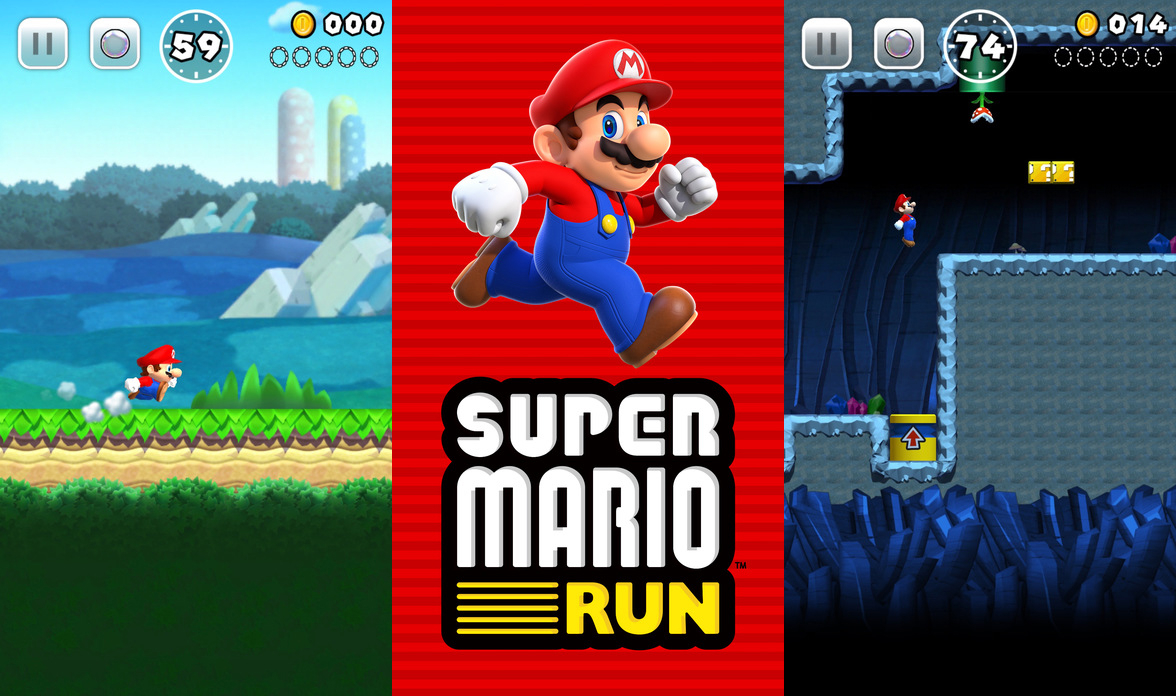
\includegraphics[scale=0.18]{figures/UIDesign/Superm.jpg}
\caption{Screenshots of the game SUPER MARIO RUN}
\label{fig1}
\end{figure}


Although there are lots of applications related to the health and especially personal health companions and helps if you're having small health issues, ``ZenZe'' has its reason to exist . For example 'ADA' is an app that can understand what is wrong if you are not feeling well. By engaging in a private conversation with you, ADA can help you with personalized answers. There are also a lot of games related to surgery, to give interest to young children in learning from these jobs or to give the desire to learn more about the human body. And finally, we can find many applications about brain training games to improve the memory, attention, accuracy and logic skills. Thus we find a large number of applications on the play store linked with the health and the mental illnesses. However the features of these applications stop either to a list of information or to a memory or logic games. Our application is different from others in the sense that it allows the user to be both active and responsive through playing, and has a series of features that encourage the user to share disease information with others. Thanks to this our application allows the patients an opening on the world and avoids loneliness. When compared with other health Apps, ``ZenZe'' shows its difference significantly. Most professional healthy Apps just provide solution about user's physical health. For example, Some fitness apps provide some fitness instructional videos to teach the user the correct action to do when exercising and others have the ability to use gauges and loggers as sensors to measure numbers of steps during a period.

The main difference between ``ZenZe'' and other health Apps is the different goals of them. Common health Apps are mainly focusing on the physical health issues but not mental health. ``ZenZe'' tries to do something on people's mental health. Most people's mood are influenced by weather, for example, most people like sunny weather, if it is sunny, ``ZenZe'' will show ''sunny mode'' to player, then the player can enjoy the advantages of sunny weather, just like feeling the sunlight through ``ZenZe'', on the other hand, if the weather is bad, people may release their induced stress by playing ``ZenZe'' (don't forget ``ZenZe'' is a game, therefore it's here for the user's entertainment).

In sum, when compared with three different kinds of Apps, ``ZenZe'' has its shortages and advantages. It always has some very good  features that other Apps do not have, which makes ``ZenZe'' different from most other Apps. 

\section{Literature review}
In recent years, more and more researchers have used their mobile device as tools for heath care \cite{ventolal} \cite{healthcarepocket}. A mobile phone has been regarded as a platform of improvement for people's health. In this platform, researchers developed different kinds of Apps to make interactions between human beings and mobile devices, in order to 'supervise' people's health \cite{healthcarepocket}. For example, researchers developed step-counter Apps to improve the level of people's physical health by the visualization of the exercising habits of a population \cite{stepup}. During the process of developing Apps, sensors were convenient tools, and made those Apps more interesting. The main ideas behind most research is always more or less the same: Health is displayed by visualizing strength and ''performance'' of one's body but not his mentality; people's health can be changed through some operations on two things - ''diets and exercises''. Even though there are some apps that are designed for mental health \cite{devmental}, when comparing with apps focusing on physical health, we find out that they are much less of them.  
From these research papers above, we thought we could also make an App which focuses on people's health, and this App should be using sensors. However, we decided to make this app for people's mental health and not their physical one; and we planned to use some sensors not for counting anything, but for other operations.
In addition, with the development of software and  hardware on mobile phones, it is getting easier to develop a mobile phone game. Many researchers have already used mobile phone games as a treatment to physical health issues \cite{seriousgames} \cite{seriousgameshealth}. Some games use a number of strategies to invoke people's motivation to do exercise which aims at promoting their physical health. Now that game can invoke people's motivation, it should be able to change people's mental status. Moreover, one of the natural features of a game is making people relaxed.  Therefore, making a game to aiming at people's mental health is an ideal choice.
To summarize, apps for physical are not uncommon, and it is common to use sensors in them. Many games are currently focusing on physical health and they can use some methods to change people mental status (with motivation). From these points, we decided to use some sensors in our Apps, not for improving people's physical health but to improve their enjoyment of our application. The App's goal is to improve the users' mental health by changing their mental status, and the App would be designed as a game.


\section{Originality}
One of the most valuable aspects of an app is its originality. In this section, we illustrate its uniqueness in terms of app design, game controls and developing purposes.
\subsection{App Design}
In the APP design session, we call a weather service and location service, so that we can get the local weather information in App. In this aspect, the APP is a weather-detection app. However, the most important part of this app is the game, and the change of real-time weather can change game-modes, so we can think of this APP as a game that can detect the weather. The combination of game and weather detection enabled the app to be original in the aspect of design. We put two existing things into one, and the new one consists of both key advantages of the old two Apps.

\subsection{Game Controls}
In the aspect of game controls, when comparing with other games, ``ZenZe'' is new and advanced. In most platform games, users control the character's movement by clicking different button on the screen, for example, if users want to make the character go ahead, they may click the forward button on the screen, and there are no sensor get involved in the process of moving the character. 
In contrast, when a user plays ``ZenZe'', he or she must tilt the device to make the character move forward or backwards. In this process, two sensors are used. It may make ``ZenZe'' a little more difficult for users to control the character when they are new to this game, but the increased difficulty can be regarded as more enjoyment for the player. Those sensors make ``ZenZe'' much more advanced than other sensor-less platform games, and also make ``ZenZe'' unique in the aspect of game controls.

\subsection{Fine-tuned design for users}
Thanks to a sleek design (Figure 2) and a logical sequence between the different activities, our application can quickly conquer many users. The originality of the application is really the link of affection that the user can have with this famous characters too cute that accompanies and guides the user throughout the game. The automatic location, and Facebook status sharing features provide a real connection between the user and the application in the real world. The user can feel accompanied in his daily life by the application that adapts in real time to weather conditions for example.

To summarize, we attached advantages of two kinds of Apps to one App, and made it into a new App. The new one has more than one original features, and these original features can be merged together perfectly, but no one has done that before. So we decided to do so.

\section{Targeted Users}
``ZenZe'' combines both platform games and weather app, and its main goal is trying to improve people's mental status to. It is aimed towards both kids and adults for them to entertain themselves on a long rainy day, or a boring sunny one.

\begin{figure}[!tb]
\centering
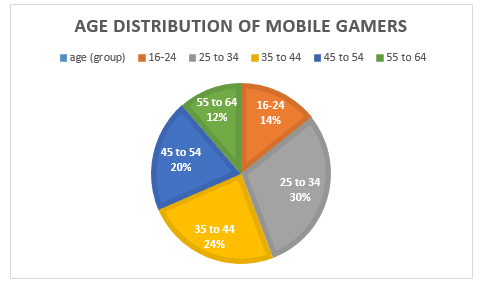
\includegraphics[scale=0.80]{figures/agedist.png}
\caption{Age distribution of mobile gamers}
\label{fig2}
\end{figure}

``ZenZe'' suits all kinds of users in different age periods. People's mood are fragile and influenced by weather, no matter how old they are; people in all ages should know local weather to make some decisions like whether to take umbrella when going  outside. However, to make ``ZenZe'' more popular, we searched for the age distribution of mobile gamers. As we can see in Figure 2, the number of players who age from 25 to 34 has the most proportion of  mobile users, then are people who are from 35 to 44. Therefore, the target users of ``ZenZe'' are people whose age are from 25 to 44 (cf. figure 2).

\section{key Design}

\subsection{Description of design consideration}

The application consists of seven different views in total. An overview of these views and the transitions between them is given in figure 3 %\ref{fig:storyboard}.
At the beginning you see a \textbf{main menu} with the options to start the game, read the instructions on how to play and adapt some settings.

The \textbf{game view} contains the current level and some important information about the gameplay like health and attacks available. The game dynamics are as follows: The state of the game changes based on the weather. In the current configuration it supports the three states sunny, rainy and snowy. The user can move the avatar by tilting the mobile device to the left or to the right. To jump the left side of the screen has to be touched and to attack the right side. The height of the jump can be controlled by the length of the touch, but is limited to a maximum jump-time.

The player has one standard attack, but can gain special attacks by defeating enemies. These special attacks come in three categories reflecting the three game states and give the player a certain bonus or malus depending on the type of enemy it is used against. As these attacks are more useful against enemies in a different state, the player is encouraged to wait for the weather status to change throughout the level.

During a level the player can also collect various pick-up items. Whenever a new item or enemy is encountered a message pops up giving the user the option to view more detailed information about this item or enemy. By clicking onto \textit{some symbol next to the players health bar} the user can review statistics like which items he/she already collected.





\begin{figure*}
\centering
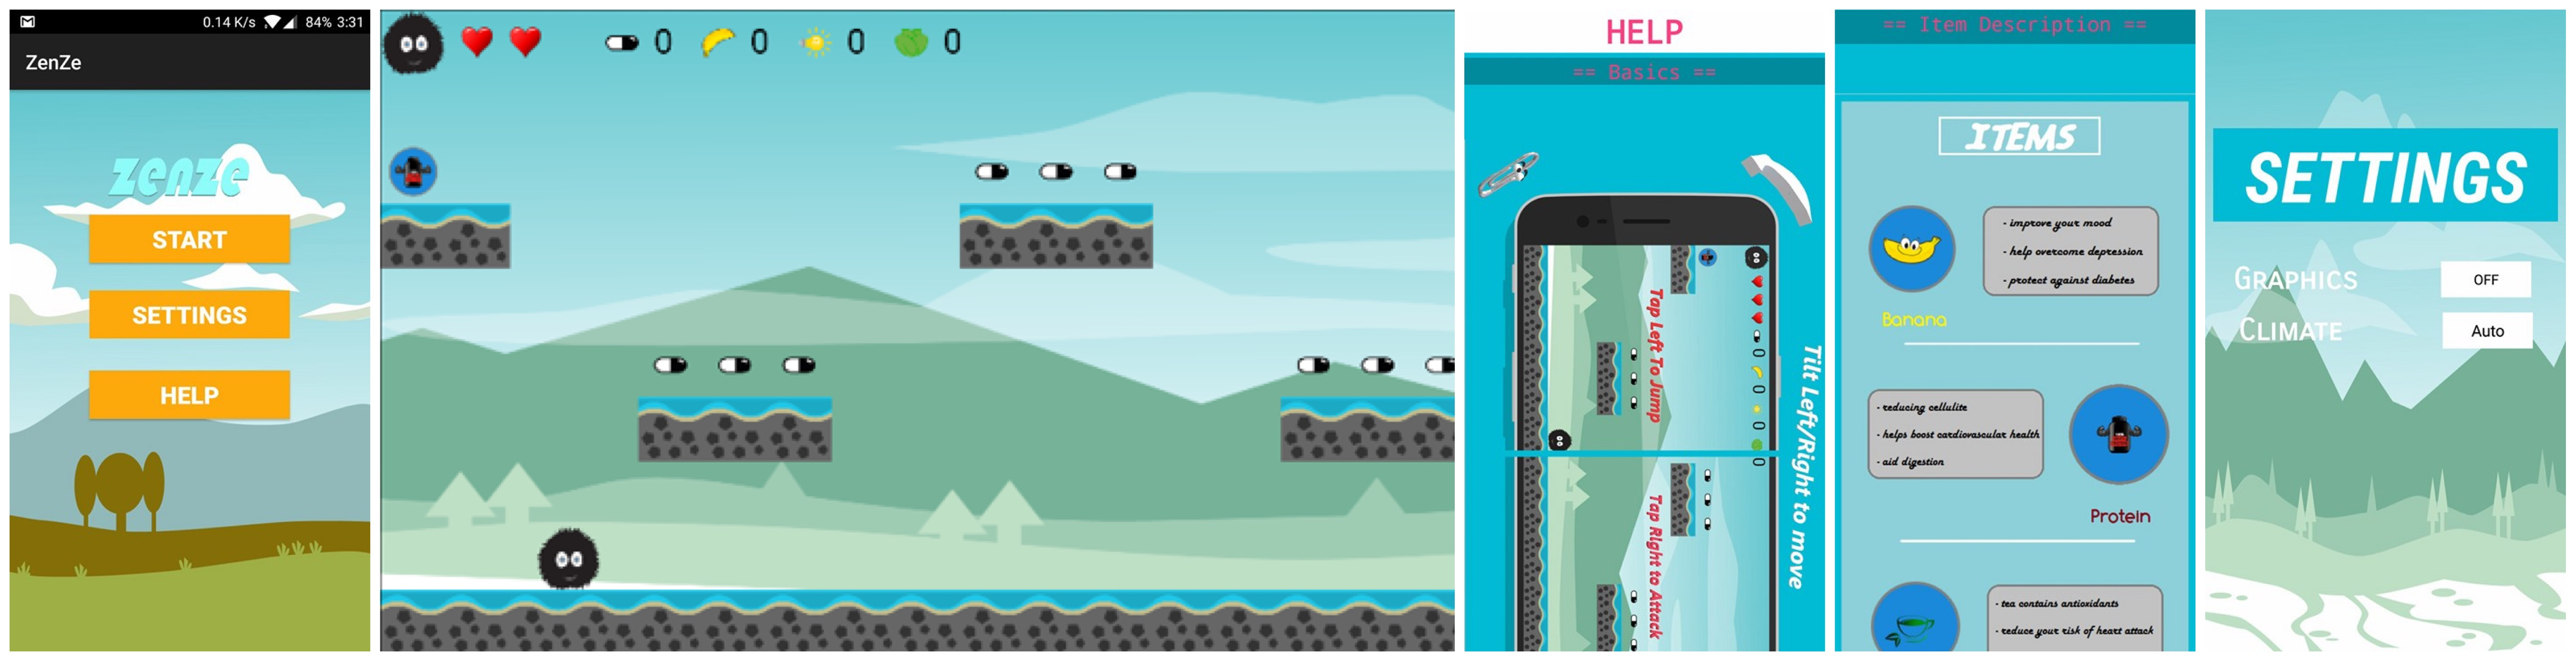
\includegraphics[width=7in]{figures/zenzescreenshot.jpg}
\caption{Some screen shots of ZenZe}
\label{fig3}
\end{figure*}




\begin{figure*}
\label{fig:storyboard}
	\centering
	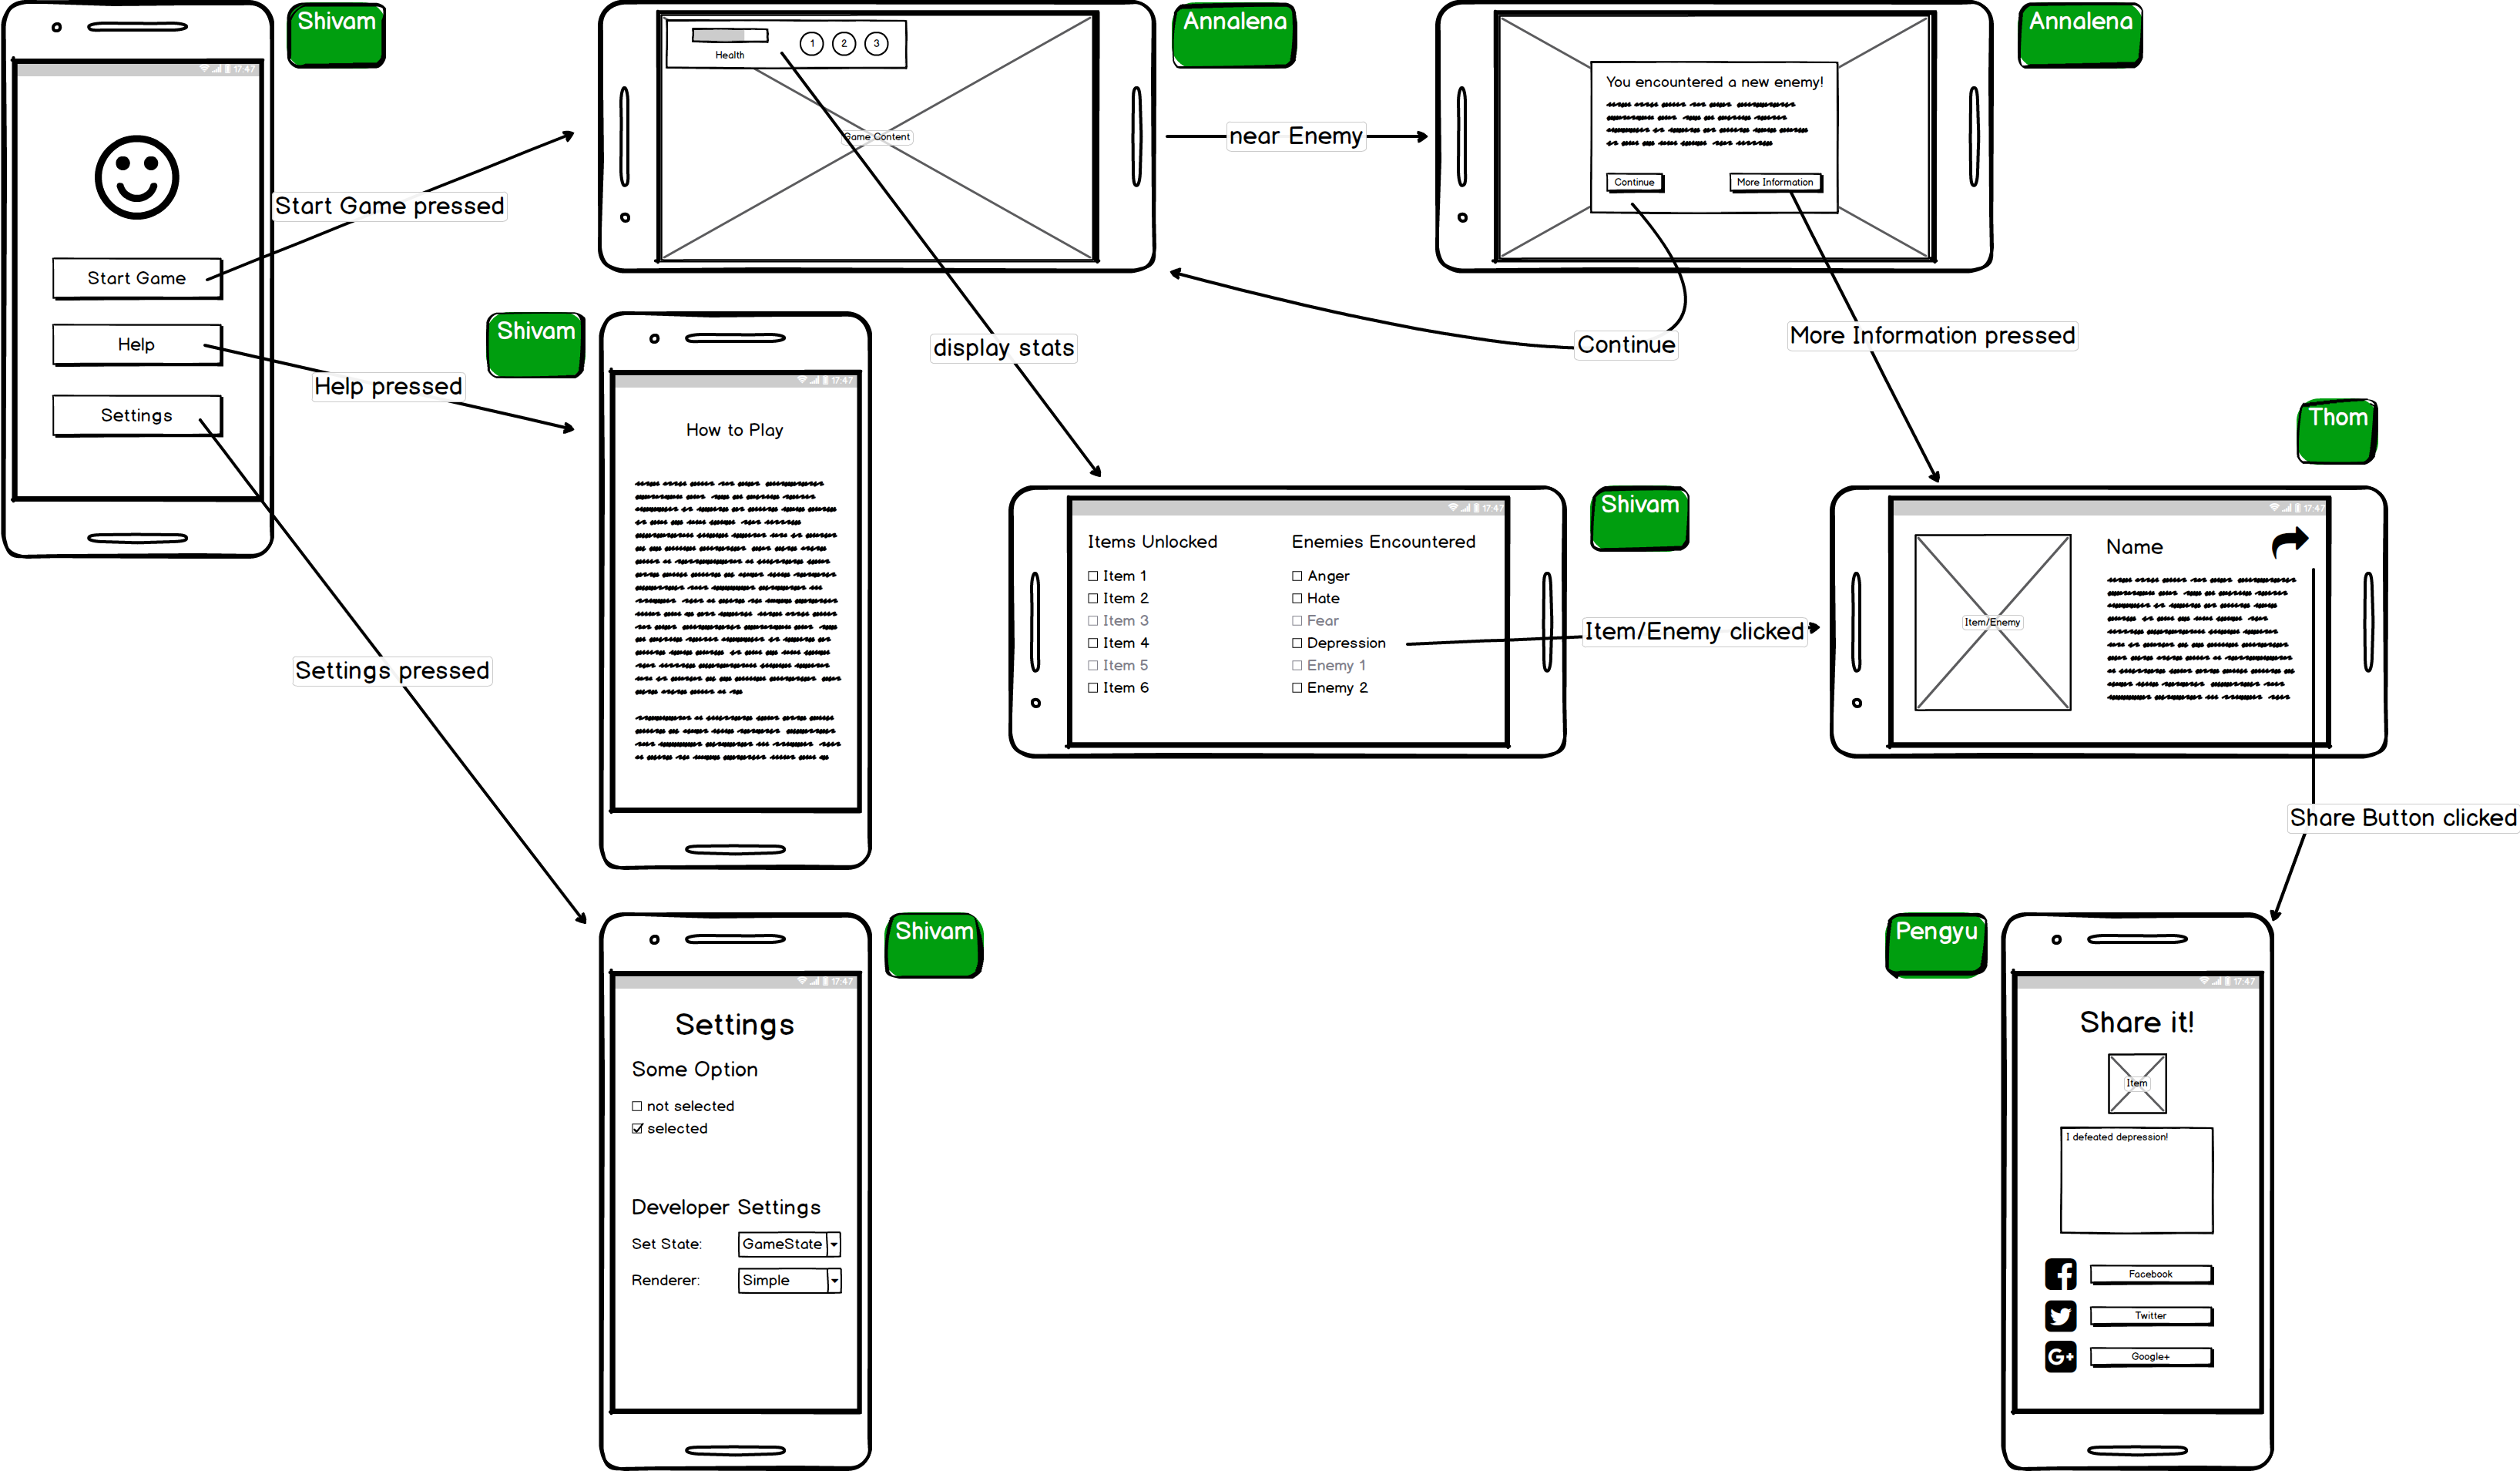
\includegraphics[width=7in]{figures/UIDesign/Storyboard.png}
	\caption{A storyboard of the app created with Balsamiq Mockups}
\end{figure*}



\subsection{Key Use Cases}
When users play ``ZenZe'', they need rotate or incline their phones or tablets to make the character run. This requires users move their devices during the process of operating the character and pay attention to their screens,  so users should focus on ``ZenZe'' when they play it, and not have other things to do. 
The perfect period to play ``ZenZe'' is playing ``ZenZe'' after you wake up but before get up at morning. Just imagine,  when you just woke up, you may feel very sleepy, but if you play ``ZenZe'', which requires for you to pay attention to it with moving your device to move the character around, it will help you wake up. Meanwhile, because you have not open the curtains yet, you do not know what is the weather outside, so you do not know how to dress today, whether you should dress with light or heavy clothes, ``ZenZe'' will inform you on the weather!


\section{Implementation}

This section will go more in detail on what we've built and how we've built it in regards to the Zen-Ze application. We won't cover the code in detail but we will focus on architecture and design.

For the full source code please refer to \url{https://github.com/Zen-Ze/ZenZe}.

\subsection{Key Features \& Technical Achievements}
Our application being a game, there are quite a few aspects we had to cover in terms of Game Design. For this we used the phone sensors (in particular the gyroscope) which makes the main character move around the map. Additionally, tapping on the right or on the left of the screen will trigger either the jump or the attack of the character. 

Additionally, we decided to implement a database with our application. We wanted to have a simple and effective way of storing data from the application directly on the phone. For this we used the built-in SQLITE database that comes with Android. To implement this database in our application, we created a back-end package and added a library (the room persistence library \url{https://developer.android.com/topic/libraries/architecture/room.html}) to the project. The library in itself helped us create an interface between the Java application and the SQL. In this library, we define models (named entities), which are Java objects to which the data from the tables in the database will be transformed, but also Daos which are interfaces to create CRUD (create, read, update, delete) operations for our objects in the database. As for the database scheme, please find it enclosed at the end of the document.

Another key feature is the use of the OpenWeatherMap API. Our application relies on the weather and displays graphics based off it. For this we thus had to use some sort of service which would give us the weather and from this service inform the application. We used the OpenWeatherMap API for that as it's an API we had used in class and it seemed to fit our needs. One of the limitations with this API is though that we will not be able to publish the application to the play store, unless we pay OpenWeatherMap to be allowed to do more daily queries to the API. 

Finally, a key feature we added was the GPS. This was required for the weather service to be called properly as we queried the weather using the longitude and latitude of a location. For this we used the google play services library (\url{https://developer.android.com/training/location/index.html}) in order to retrieve a Location object of the last known location when the app is launched. 


\begin{figure*}
\label{fig:dbscheme}
	\centering
	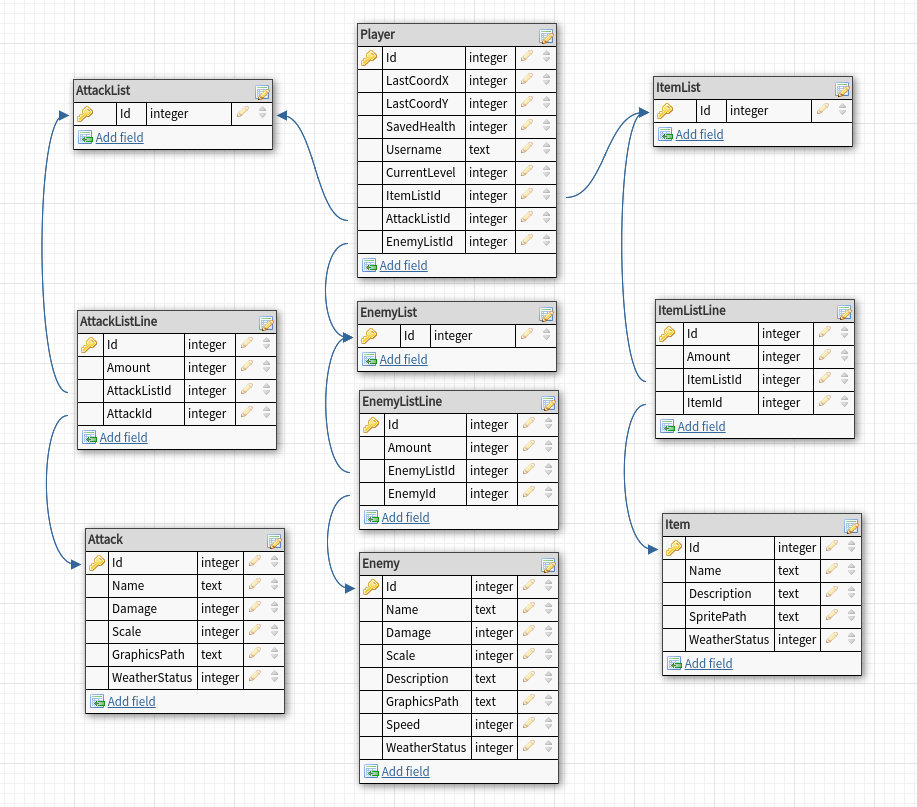
\includegraphics[width=7in]{figures/UIDesign/DBScheme.png}
	\caption{Database Scheme} 
\end{figure*}

\subsection{Key Lessons}
In this project, we have learned many things, in terms of coding for android, designing an application from scratch, understanding the concepts behind android... Out of all we learned, there are noticeable lessons we've gathered from this project. 

The first noticeable one was to comment our code properly so others could read and understand it, either with checking the files or by reading through the generated documentation. Additionally, we've learned to work as a team on different parts of the application, thus communication was key throughout the project.
Another part in which we learned a lot was with the overall design thinking process with each members finding 10 different ideas and gathering them to find the best one of them all.

\section{Project closeout}

%\begin{figure}
%\label{fig:figure1}
%\centering
%  
\includegraphics[width=0.9\columnwidth]{figures/sigchi-logo}
%  \caption{caption}
%\end{figure}
%
%This is a citation~\cite{acm_categories,ethics,Klemmer:2002:WSC:503376.503378}.\\
%This is a reference~\ref{fig:figure1}.\\
%This is a link \url{http://chi2016.acm.org/accessibility}.\\
%This is a ''quotation''.\\
%
%\begin{quote}
%This is a longer quote.  
%\end{quote}
%
%\begin{table}
%  \centering
%  \begin{tabular}{l r r r}
%    % \toprule
%    & & \multicolumn{2}{c}{\small{\textbf{Test Conditions}}} \\
%    \cmidrule(r){3-4}
%    {\small\textit{Name}}
%    & {\small \textit{First}}
%      & {\small \textit{Second}}
%    & {\small \textit{Final}} \\
%    \midrule
%    Marsden & 223.0 & 44 & 432,321 \\
%    Nass & 22.2 & 16 & 234,333 \\
%    Borriello & 22.9 & 11 & 93,123 \\
%    Karat & 34.9 & 2200 & 103,322 \\
%    % \bottomrule
%  \end{tabular}
%  \caption{Table caption}~\label{tab:table1}
%\end{table}
%
%\begin{itemize}
%\item item 1
%\item item 2
%\end{itemize}
%
%\begin{enumerate}
%\item enum 1
%\item enum 2
%\end{enumerate}

\subsection{Result of the final App}
Our application meets most of the standards we had defined at first. After opening ``ZenZe'', there are three buttons: start, settings and help, and after the start button being clicked, the game will start. When a player encounters a new item, they can read out the description of it, and learn the benefits associated with it. Users can also change the game-mode by clicking on the ''settings'' button, the default setting is ''Change by real-time weather''.If an user want to share the fact that he's using our application on Facebook, he or she may login Facebook firstly, and then he or she can share something of ``ZenZe'' to his or her timeline on Facebook. When users click on the ''help'' button, they get access to a guide which tells them how to play the game. A part of features are shown as figure 3, which are some screenshots of ``ZenZe''.

\subsection{Conclusion}
This app ``ZenZe'' focuses on people's mental health, and it get some key information (weather) from the real world then applies these information into virtual world (game). In design process, we combine features of weather apps and platform games into one App and get some inspiration from Apps which focus on promoting people's health. In  the whole process of developing ``ZenZe'', we used databases, OpenWeatherMap API, the GPS, and other sensors to improve its performance and flow. The application we developed seems to meet what we had planned at first. The most obvious advantage of ``ZenZe'' is  the idea of relation between a virtual environment and the real world, and some sensors in ``ZenZe'' make it more interesting for the user than other platform games. However, there are many aspects of the application which could be improved. For example, the share function could allow the user to share data to more social media than facebook, the graphics renderer could be faster if we used a library instead of the built-in android canvas, we could add extra levels and we could try to make it a 3D game which would make the game more interesting. 


\section{Acknowledgments}
We thank each team members who took part in the process of developing ``ZenZe'', thank our classmates who gave us some help and inspiration, and authors of materials that we referenced for making ``ZenZe''. Finally we thank our lecturer, who taught us knowledge in class, and grouped us at random, made us from strangers to teammates to friends. Through this period of application development, we not only gained knowledge, but also gain friendship and the spirit of cooperation.

% Balancing columns in a ref list is a bit of a pain because you
% either use a hack like flushend or balance, or manually insert
% a column break.  http://www.tex.ac.uk/cgi-bin/texfaq2html?label=balance
% multicols doesn't work because we're already in two-column mode,
% and flushend isn't awesome, so I choose balance.  See this
% for more info: http://cs.brown.edu/system/software/latex/doc/balance.pdf
%
% Note that in a perfect world balance wants to be in the first
% column of the last page.
%
% If balance doesn't work for you, you can remove that and
% hard-code a column break into the bbl file right before you
% submit:
%
% http://stackoverflow.com/questions/2149854/how-to-manually-equalize-columns-
% in-an-ieee-paper-if-using-bibtex
%
% Or, just remove \balance and give up on balancing the last page.
%

\bibliography{references}
\bibliographystyle{SIGCHI-Reference-Format}

\end{document}
